%%%%%%%%%%%%%%%%%%%%%%%%%%%%%%%%%%%%%%%%%%%%%%%%%%%%%%%%%%%%%%%%%%%%%%%%%%%%%%%
% Titel:   Bericht - Admin
% Autor: Simon Grossenbacher  
% Datum:   27.09.2013
% Version: 1.0.1
%%%%%%%%%%%%%%%%%%%%%%%%%%%%%%%%%%%%%%%%%%%%%%%%%%%%%%%%%%%%%%%%%%%%%%%%%%%%%%%
%
%:::Change-Log:::
% Versionierung erfolgt auf folgende Gegebenheiten: -1. Release Versionen
%                                                   -2. Neue Kapitel
%                                                   -3. Fehlerkorrekturen
%
% 0.0.0       Erstellung der Datei
%
%:::Hinweis:::
% Indexerstellung: makeindex -s report.ist report.idx
%   Umlaute m�ssen separat behandelt werden!
%%%%%%%%%%%%%%%%%%%%%%%%%%%%%%%%%%%%%%%%%%%%%%%%%%%%%%%%%%%%%%%%%%%%%%%%%%%%%%%
\documentclass[version=last,fleqn,pointlessnumbers]{scrreprt}  %first: Ergebniss Kompatibel zu ersten Version; last: Ergebniss entspricht den aktuellen Paketen; fleqn: Formeln linksb�ndig; pointlessnumbers: Kapitelnummerierung ohne Punkt; twoside: Doppelseitiger Druck

%Dokumentangaben
\newcommand{\Titel}{Latex-Vorlage}
\newcommand{\Uebertitel}{Bericht}
\newcommand{\AutorA}{T\"odel 1}
\newcommand{\AutorB}{T\"odel 2}
\newcommand{\AutorC}{T\"odel 3}
\newcommand{\Dozent}{Superman}
\newcommand{\Klasse}{The Fantastic}
\newcommand{\Datum}{\today}
\newcommand{\Ort}{Burgdorf}
\newcommand{\Version}{1.0.1}



%%%%%%%%%%%%%%%%%%%%%%%%%%%%%%%%%%%%%%%%%%%%%%%%%%%%%%%%%%%%%%%%%%%%%%%%%%%%%%%
% Pakete
%%%%%%%%%%%%%%%%%%%%%%%%%%%%%%%%%%%%%%%%%%%%%%%%%%%%%%%%%%%%%%%%%%%%%%%%%%%%%%%
%%%%%%%%%%%%%%%%%%%%%%%%%%%%%%%%%%%%%%%%%%%%%%%%%%%%%%%%%%%%%%%%%%%%%%%%%%%%%%%
% Titel:   Bericht - Pakete
% Autor: Simon Grossenbacher  
% Datum:   27.09.2013
% Version: 1.0.0
%%%%%%%%%%%%%%%%%%%%%%%%%%%%%%%%%%%%%%%%%%%%%%%%%%%%%%%%%%%%%%%%%%%%%%%%%%%%%%%
%
%:::Change-Log:::
% Versionierung erfolgt auf folgende Gegebenheiten: -1. Release Versionen
%                                                   -2. Neue Kapitel
%                                                   -3. Fehlerkorrekturen
%
% 0.0.0       Erstellung der Datei
%
%:::Hinweis:::
% Indexerstellung: makeindex -s report.ist report.idx
%   Umlaute m�ssen separat behandelt werden!
%%%%%%%%%%%%%%%%%%%%%%%%%%%%%%%%%%%%%%%%%%%%%%%%%%%%%%%%%%%%%%%%%%%%%%%%%%%%%%%

%Sprach-Optionen
\usepackage[ngerman]{babel} %neue deutsche Rechtschreibung
\usepackage[T1]{fontenc}  %richtige Worttrennung
%\usepackage[applemac]{inputenc}				% Mac - load extended character set (ISO 8859-1)
\usepackage[latin1]{inputenc}  				% Unix/Linux - load extended character set (ISO 8859-1)
%\usepackage[ansinew]{inputenc}  				% Windows - load extended character set (ISO 8859-1)
%\usepackage[utf8]{inputenc}  					% UTF-8 encoding

%Zeilenabstand
\usepackage{setspace}

%Mehr Tabellenoptionen
\usepackage{tabularx}
\usepackage{longtable}

%Besserer Flattersatz
\usepackage{ragged2e}

%Gleiten verhindern
\usepackage{float}
\usepackage{placeins}

%Ueberschriften anpassen
\usepackage{titlesec} 

%Farben
\usepackage{color}
\usepackage{colortbl} %F�r farbige Tabellen

%PDF zu Dokument hinzufuegen
\usepackage[final]{pdfpages}

%Grafiken verwalten
\usepackage{graphicx}
\usepackage[absolute]{textpos}

%Zeichnen
%\usepackage{pst-pdf}
%\usepackage{pst-all}

%Listnings verwalten
\usepackage{listings}

%Kopf- Fusszeile (Optionen m�ssen direkt �bergeben werden)
\usepackage[automark, %Automatisches aktualisieren der Chapter-Titel
%            headsepline,  %Linie Kopfzeile
%            footsepline,  %Linie fusszeilezeile
%            markuppercase,
            plainfootsepline  %Plain-Style auch mit Linie versehen
            ]{scrpage2}

%Flexible Argumente bei Funktionen
\usepackage{xargs}

%erweiterte Steuerfunktionen
\usepackage{ifthen}

%Index f�r Stichwortverzeichnis
\usepackage{makeidx}

%Index f�r Literaturverzeichnis
\usepackage[babel,german=quotes]{csquotes}
%\usepackage[backend=biber,style=numeric,defernumbers=true,sorting=nyt]{biblatex}
\usepackage[backend=bibtex,defernumbers=true]{biblatex}
\bibliography{bibliography}
\defbibheading{lit}{\section{Literatur}}
\defbibheading{pic}{\section{Abbildungen}}

%Zusaetzliche Symbole direkt im Text
\usepackage{textcomp}
\usepackage{amssymb}

%Einheit kontrolliert eingeben
\usepackage{units}

%dynamische Datumsausgabe
\usepackage[german]{isodate}

%Zusaetzlich Mathemtiksymbole
\usepackage{amsmath}
\usepackage{mathtools}

%Besser Handling von internen Countern und Berechnungen
\usepackage{calc}

%TODOs anbringen am Rand
\usepackage{todonotes}

%Hyperlinks (Muss das letzte geladene Paket sein)
\usepackage[bookmarks=true, %Verzeichnis generieren
            bookmarksopen=true, %Verzeichnis �ffnen
            bookmarksopenlevel=3, %Tiefe der Verzeichnis�ffnung
            unicode=false, %non-Latin Zeichen
            pdftoolbar=true, %PDF-Viewer Toolbar
            pdfmenubar=true, %PDF-Viewer Men�?
            pdffitwindow=true, %Fenster an Seite anpassen beim �ffnen
            pdftitle={\Titel}, %Titel
            %pdfauthor={\Autor1, \Autor2, \Autor3}, %Autor
            pdfsubject={\Uebertitel}, %Thema
%            pdfcreator={\Autor1, \Autor2, \Autor3}, %Ersteller des Dokuments
%            pdfproducer={\Autor1, \Autor2 \Autor3}, %Produzent des Dokuments
            pdfnewwindow=true, %Links in neuem Fenster
            colorlinks=true, %false: Boxen-Links; true: Farben-Links
            linkcolor=black, %Farbe von internen Links
            citecolor=black, %Farbe von Links zu Bibliography
            filecolor=magenta, %Farbe von Links zu Dateien
            urlcolor=blue %Farbe von externen Links
            ]{hyperref}




%%%%%%%%%%%%%%%%%%%%%%%%%%%%%%%%%%%%%%%%%%%%%%%%%%%%%%%%%%%%%%%%%%%%%%%%%%%%%%%
% Funktionen
%%%%%%%%%%%%%%%%%%%%%%%%%%%%%%%%%%%%%%%%%%%%%%%%%%%%%%%%%%%%%%%%%%%%%%%%%%%%%%%
%%%%%%%%%%%%%%%%%%%%%%%%%%%%%%%%%%%%%%%%%%%%%%%%%%%%%%%%%%%%%%%%%%%%%%%%%%%%%%%
% Titel:   Bericht - Funktionen
% Autor:   Simon Grossenbacher  
% Datum:   27.09.2013
% Version: 1.0.0
%%%%%%%%%%%%%%%%%%%%%%%%%%%%%%%%%%%%%%%%%%%%%%%%%%%%%%%%%%%%%%%%%%%%%%%%%%%%%%%
%
%:::Change-Log:::
% Versionierung erfolgt auf folgende Gegebenheiten: -1. Release Versionen
%                                                   -2. Neue Kapitel
%                                                   -3. Fehlerkorrekturen
%
% 0.0.0       Erstellung der Datei
%
%:::Hinweis:::
% Indexerstellung: makeindex -s report.ist report.idx
%   Umlaute m�ssen separat behandelt werden!
%%%%%%%%%%%%%%%%%%%%%%%%%%%%%%%%%%%%%%%%%%%%%%%%%%%%%%%%%%%%%%%%%%%%%%%%%%%%%%%

%%%%%%%%%%%%%%%%%%%%%%%%%%%%%%%%%%%%%%%%%%%%%%%%%%%%%%%%%%%%%%%%%%%%%%%%%%%%%%%
% Text tiefstellen
% param #1 Text
%%%%%%%%%%%%%%%%%%%%%%%%%%%%%%%%%%%%%%%%%%%%%%%%%%%%%%%%%%%%%%%%%%%%%%%%%%%%%%%
\newcommand{\low}[1]{\textsubscript{#1}}



%%%%%%%%%%%%%%%%%%%%%%%%%%%%%%%%%%%%%%%%%%%%%%%%%%%%%%%%%%%%%%%%%%%%%%%%%%%%%%%
% Text hochstellen
% param #1 Text
%%%%%%%%%%%%%%%%%%%%%%%%%%%%%%%%%%%%%%%%%%%%%%%%%%%%%%%%%%%%%%%%%%%%%%%%%%%%%%%
\newcommand{\high}[1]{\textsuperscript{#1}}



%%%%%%%%%%%%%%%%%%%%%%%%%%%%%%%%%%%%%%%%%%%%%%%%%%%%%%%%%%%%%%%%%%%%%%%%%%%%%%%
% Schrift anpassen
% param #1 Schriftfamilie: ptm  Times
%                          phv 	Helvetica
%                          pcr 	Courier
%                          pbk 	Bookman
%                          pag 	Avant Garde
%                          ppl 	Palatino
%                          pch 	Charter
%                          pnc 	New Century Schoolbook
%                          put 	Utopia
% param #2 Strichdicke/Zeichenbreite: b  bold
%                                     m  medium
% param #3 Schriftform: n   normal
%                       it  italic
%                       sl  slanted
%                       sc  small caps
%                       ui  upright italic
% note {\changefont{#1}{#2}{#3} Hallo Welt} Teilbereich aendern
%%%%%%%%%%%%%%%%%%%%%%%%%%%%%%%%%%%%%%%%%%%%%%%%%%%%%%%%%%%%%%%%%%%%%%%%%%%%%%%
\newcommand{\changefont}[3]{\fontfamily{#1} \fontseries{#2} \fontshape{#3} \selectfont}



%%%%%%%%%%%%%%%%%%%%%%%%%%%%%%%%%%%%%%%%%%%%%%%%%%%%%%%%%%%%%%%%%%%%%%%%%%%%%%%
% Zum Beispiel abkuerzen ohne Trennung
% param none
%%%%%%%%%%%%%%%%%%%%%%%%%%%%%%%%%%%%%%%%%%%%%%%%%%%%%%%%%%%%%%%%%%%%%%%%%%%%%%%
\newcommand{\zB}{z.~B.}



%%%%%%%%%%%%%%%%%%%%%%%%%%%%%%%%%%%%%%%%%%%%%%%%%%%%%%%%%%%%%%%%%%%%%%%%%%%%%%%
% Formeleintrag
% param #1 Formel
% param #2 Parameter Beschreibung im Tabellensyntax
% param #3 Formel-Label (optional)
%%%%%%%%%%%%%%%%%%%%%%%%%%%%%%%%%%%%%%%%%%%%%%%%%%%%%%%%%%%%%%%%%%%%%%%%%%%%%%%
%Savebox fuer Parameterbeschreibung
\newsavebox{\myendhook} % for the tabulars
\makeatletter
\def\tagform@#1{{(\maketag@@@{\ignorespaces#1\unskip\@@italiccorr)}
\makebox[0pt][r]{% after the equation number
\makebox[0.5\textwidth][l]{\usebox{\myendhook}}%
}%
\global\sbox{\myendhook}{}% clear box content
}}
\makeatother 
%Kommando definieren
\newcommandx{\formula}[3][3=\empty,usedefault]{
    \sbox{\myendhook}{%
        \begin{footnotesize}%
            \begin{tabular}{@{}l >{\RaggedRight}p{.33\textwidth}}%0.33
                #2%\ifthenelse{\equal{#2}{\empty}}{ }{#2}
            \end{tabular}
        \end{footnotesize}}
    %
    \begin{equation}
        \ifthenelse{\equal{#3}{\empty}}
        {}
        {\label{#3}}%anstatt equation	
        \boxed{\begin{split}#1\end{split}}
        %\begin{split}#1\end{split}
    \end{equation} %anstatt equation
}



%%%%%%%%%%%%%%%%%%%%%%%%%%%%%%%%%%%%%%%%%%%%%%%%%%%%%%%%%%%%%%%%%%%%%%%%%%%%%%%
% Bildereintrag
% param #1 Pfad zum Bild
% param #2 Groesse: z.B. scale=0.5
% param #3 Bildunterschrift (optional)
% param #4 Bildunterschrift im Abbildungsverzeichnis (optional)
% param #5 Bildlabel (optional)
%%%%%%%%%%%%%%%%%%%%%%%%%%%%%%%%%%%%%%%%%%%%%%%%%%%%%%%%%%%%%%%%%%%%%%%%%%%%%%%
\newlength{\imagewidth}
\newlength{\imageheight}
\newcommandx{\image}[5][3=\empty,4=\empty:,5=\empty,usedefault]{
    \begin{figure}[H]%H htbp
        \centering
        \settowidth{\imagewidth}{\includegraphics[#2]{#1}}
        \settoheight{\imageheight}{\includegraphics[#2]{#1}}
        \ifdim\imagewidth<\textwidth
            \ifdim\imageheight<\textheight
                \includegraphics[#2]{#1}
            \else
                \includegraphics[height=\textheight]{#1}
            \fi
        \else
            \ifdim\imageheight<\textheight
                \includegraphics[width=\textwidth]{#1}
            \else
                \setlength{\imageheight}{\imageheight-\textheight}
                \setlength{\imagewidth}{\imagewidth-\textwidth}
                \ifdim\imageheight<\imagewidth
                    \includegraphics[width=\textwidth]{#1}
                \else
                    \includegraphics[height=\textheight]{#1}
                \fi
            \fi
        \fi
        \ifthenelse{\equal{#5}{\empty}}
        {
            \ifthenelse{\equal{#3}{\empty}}{}{\caption{#3}}
            \ifthenelse{\equal{#4}{\empty}}{}{\label{#4}}
        }
        {
            \caption[#4]{#3}
            \label{#5}
        }
    \end{figure}
}



%%%%%%%%%%%%%%%%%%%%%%%%%%%%%%%%%%%%%%%%%%%%%%%%%%%%%%%%%%%%%%%%%%%%%%%%%%%%%%%
% Bildereintrag fuer Tabellen
% param #1 Pfad zum Bild
% param #2 Groesse: z.B. scale=0.5
%%%%%%%%%%%%%%%%%%%%%%%%%%%%%%%%%%%%%%%%%%%%%%%%%%%%%%%%%%%%%%%%%%%%%%%%%%%%%%%
\newlength{\myx} % Variable zum Speichern der Bildbreite
\newlength{\myy} % Variable zum Speichern der Bildh�he
\newcommand{\imagetotab}[2][\relax]{%
% Abspeichern der Bildabmessungen
\settowidth{\myx}{\includegraphics[{#1}]{#2}}%
\settoheight{\myy}{\includegraphics[{#1}]{#2}}%
% das eigentliche Einf�gen
\parbox[c][1.1\myy][c]{\myx}{%
\includegraphics[{#1}]{#2}}%
}




%%%%%%%%%%%%%%%%%%%%%%%%%%%%%%%%%%%%%%%%%%%%%%%%%%%%%%%%%%%%%%%%%%%%%%%%%%%%%%%
% Farben
%%%%%%%%%%%%%%%%%%%%%%%%%%%%%%%%%%%%%%%%%%%%%%%%%%%%%%%%%%%%%%%%%%%%%%%%%%%%%%%
\RequirePackage{color}                        	% Color (not xcolor!)
%Allgemein
\definecolor{grey}{gray}{0.7}
\definecolor{lightgrey}{gray}{0.9}

%BFH
\definecolor{bfhred}{rgb}{0.776,0,0.066}
\definecolor{brickred}{cmyk}{0,0.89,0.94,0.28}	% Brickred
\definecolor{bfhblue}{rgb}{0.396,0.49,0.56}  		% Blue
\definecolor{bfhorange}{rgb}{0.961,0.753,0.196}  	% Orange
\definecolor{bfhorangelight}{RGB}{246,216,136}  	% Orange Light

%Listing
\definecolor{hellgelb}{rgb}{1,1,0.8}
\definecolor{listingbackground}{RGB}{246,216,136} 
\definecolor{colKeys}{rgb}{0,0,1}
\definecolor{colIdentifier}{rgb}{0,0,0}
\definecolor{colComments}{rgb}{0.2,0.8.3}
\definecolor{colString}{rgb}{0,0.5,0}



%%%%%%%%%%%%%%%%%%%%%%%%%%%%%%%%%%%%%%%%%%%%%%%%%%%%%%%%%%%%%%%%%%%%%%%%%%%%%%%
% Schrift
%%%%%%%%%%%%%%%%%%%%%%%%%%%%%%%%%%%%%%%%%%%%%%%%%%%%%%%%%%%%%%%%%%%%%%%%%%%%%%%
%Standardschriftgr�sse
\KOMAoptions{fontsize=11pt}

%Zeilenabstand
%\onehalfspacing %1.5 Zeilenabstand

%Schrift eines bestimmten Elements anpassen/erstellen z.B. captionlabel
%\setkomafont{captionlabel}{\itshape}  %definert Schriftart f�r captionlabel
%\addkomafont{captionlabel}{\itshape}  %f�gt Eigenschaft zu captionlabel hinzu

%Formatvorlage anpassen
\setkomafont{pageheadfoot}{\footnotesize\sffamily} %Kopf-/Fusszeile \normalfont
\setkomafont{pagenumber}{\normalfont\sffamily\bfseries} %Seitennummer



%%%%%%%%%%%%%%%%%%%%%%%%%%%%%%%%%%%%%%%%%%%%%%%%%%%%%%%%%%%%%%%%%%%%%%%%%%%%%%%
% Gleitobjekte (Bilder/Tabellen/Formeln)
%%%%%%%%%%%%%%%%%%%%%%%%%%%%%%%%%%%%%%%%%%%%%%%%%%%%%%%%%%%%%%%%%%%%%%%%%%%%%%%
%Formelneinzug = wie Aufz�hlungseinzug
\setlength{\mathindent}{0.6\leftmargini}

%Gleitobjekte
\setlength{\intextsep}{8mm +2mm -2mm}%\intextsep10mm plus3mm minus2mm
%\setlength{\textfloatsep}{100mm plus5pt minus3pt}

%Bild-Tabellen Beschriftung linksb�ndig
%\KOMAoptions{captions=nooneline}  %linksb�ndig
\setcaphanging  %Mehrzeilige Beschriftung erh�lt Einzug



%%%%%%%%%%%%%%%%%%%%%%%%%%%%%%%%%%%%%%%%%%%%%%%%%%%%%%%%%%%%%%%%%%%%%%%%%%%%%%%
% Seiteneinstellungen
%%%%%%%%%%%%%%%%%%%%%%%%%%%%%%%%%%%%%%%%%%%%%%%%%%%%%%%%%%%%%%%%%%%%%%%%%%%%%%%
%Dokumentstadium
\KOMAoptions{draft=false}  %Erleichert das erkennen von Fehlern im Entwurfsstadium

%Papierformat
\KOMAoptions{paper=A4}  %Format (Bei direkten Massangaben: 5cm:3cm)
%\KOMAoptions{paper=landscape} %Ausrichtung  (Standard Portrait)
\KOMAoptions{pagesize=automedia}  %Angabe f�r Ausgangstreiber

%Bindekorrektur
%\KOMAoptions{BCOR=0.1cm}  %Bindekorrektur (Bereich der durchs Binden verloren geht)

%Gr�sse des Satzspiegels
\KOMAoptions{DIV=11}  %gr�sse des Satzspiegels (Faktor ab 4), siehe S.38 scrguide.pdf; nur f�r A4 existieren Voreinstellungen, sonst calc o. classic als Option

%Randbereich
\KOMAoptions{mpinclude=false} %Definiert ob der Randbereich zum Textk�rper hinzugez�hlt werden soll oder nicht -> TRUE nur bei Sonderf�llen

%Doppelspaltiges Dokument
\KOMAoptions{twocolumn=false}

%Absatzabstand
\KOMAoptions{parskip=true}

%Seitenstyle
\pagestyle{scrheadings} %myheadings scrheadings

%Platzierzung letzte Zeile
\raggedbottom %Letze Zeile liegt dort wo sie gerade ist -> unterschiedlicher vertikaler Abstand zu Blatt Ende (unerw�nscht bei doppelseitigem Druck)
%\flushbottom  %Letze Zeile immer am Schluss -> evtl. unterschiedliche Absatzabst�nde



%%%%%%%%%%%%%%%%%%%%%%%%%%%%%%%%%%%%%%%%%%%%%%%%%%%%%%%%%%%%%%%%%%%%%%%%%%%%%%%
% Kopf-/Fusszeile
%%%%%%%%%%%%%%%%%%%%%%%%%%%%%%%%%%%%%%%%%%%%%%%%%%%%%%%%%%%%%%%%%%%%%%%%%%%%%%%
%Kopfzeile
%\clearscrheadfoot %Alle Vorgaben l�schen (plain und scrheadings)
\renewcommand*{\chaptermarkformat}{% headmark ohne Kapitelnummer
%\chapappifchapterprefix{\ }\thechapter\autodot\enskip
}
\ihead[]{\textcolor{bfhblue}{\headmark}} %Chapter Titel in Kopfzeile
\chead[]{}
\ohead[]{\textcolor{bfhblue}{\Titel}} %Titel in Kopfzeile

%Fusszeile
\ifoot[\textcolor{bfhblue}{Berner Fachhochschule}]{\textcolor{bfhblue}{Berner Fachhochschule}} %plain und scrheadings mit Dokumenttitel versehen
\cfoot[]{}
\ofoot[\textcolor{bfhblue}{\pagemark}]{\textcolor{bfhblue}{\pagemark}} %plain und scrheadings mit Seitennummer versehen



%%%%%%%%%%%%%%%%%%%%%%%%%%%%%%%%%%%%%%%%%%%%%%%%%%%%%%%%%%%%%%%%%%%%%%%%%%%%%%%
% Fussnote
%%%%%%%%%%%%%%%%%%%%%%%%%%%%%%%%%%%%%%%%%%%%%%%%%%%%%%%%%%%%%%%%%%%%%%%%%%%%%%%
%Fussnote
%\KOMAoptions{footnotes=multiple} %Fussnotennummern durch "," trennen



%Satzspiegel neu berechnen -> falls andere Schriftengeladen werden und/oder Zeilenabstand ver�ndert wird
\recalctypearea  



%%%%%%%%%%%%%%%%%%%%%%%%%%%%%%%%%%%%%%%%%%%%%%%%%%%%%%%%%%%%%%%%%%%%%%%%%%%%%%%
% Paket Listings Konfiguration
%%%%%%%%%%%%%%%%%%%%%%%%%%%%%%%%%%%%%%%%%%%%%%%%%%%%%%%%%%%%%%%%%%%%%%%%%%%%%%%

%XML
\lstdefinestyle{XML}{numbers=left, 
    basicstyle=\scriptsize\ttfamily,
    numberstyle=\tiny, 
    xleftmargin=0.5\leftmargin,
    xrightmargin=\rightmargin,
    numbersep=5pt,
    backgroundcolor=\color{listingbackground}, 
    breaklines=true,
    captionpos=b,
    language=XML}

%MATlAB
\lstdefinestyle{Matlab}{numbers=left, 
    basicstyle=\scriptsize\ttfamily,
    numberstyle=\tiny, 
    xleftmargin=0.5\leftmargin,
    xrightmargin=\rightmargin,
    numbersep=5pt,
    backgroundcolor=\color{listingbackground}, 
    identifierstyle=\color{colIdentifier}, %
    keywordstyle=\color{colKeys}, %
    stringstyle=\color{colString}, %
    commentstyle=\color{colComments}, %
    breaklines=true,
    captionpos=b,
    language=Matlab}

%ANSI C
\lstdefinestyle{C}{numbers=left, 
    basicstyle=\scriptsize\ttfamily,
    numberstyle=\tiny, 
    xleftmargin=0.5\leftmargin,
    xrightmargin=\rightmargin,
    numbersep=5pt,
    backgroundcolor=\color{listingbackground}, 
    identifierstyle=\color{colIdentifier}, %
    keywordstyle=\color{colKeys}, %
    stringstyle=\color{colString}, %
    commentstyle=\color{colComments}, %
    breaklines=true,
    captionpos=b,
    language=[ANSI] C}


\makeindex %Ab hier Indexieren
%%%%%%%%%%%%%%%%%%%%%%%%%%%%%%%%%%%%%%%%%%%%%%%%%%%%%%%%%%%%%%%%%%%%%%%%%%%%%%%
% Dokument Anfang
%%%%%%%%%%%%%%%%%%%%%%%%%%%%%%%%%%%%%%%%%%%%%%%%%%%%%%%%%%%%%%%%%%%%%%%%%%%%%%%
\begin{document}
%
%
%%%%%%%%%%%%%%%%%%%%%%%%%%%%%%%%%%%%%%%%%%%%%%%%%%%%%%%%%%%%%%%%%%%%%%%%%%%%%%%
% Titelseite
%%%%%%%%%%%%%%%%%%%%%%%%%%%%%%%%%%%%%%%%%%%%%%%%%%%%%%%%%%%%%%%%%%%%%%%%%%%%%%%
%%%%%%%%%%%%%%%%%%%%%%%%%%%%%%%%%%%%%%%%%%%%%%%%%%%%%%%%%%%%%%%%%%%%%%%%%%%%%%%
% Titel:   Titelseite
% Autor:   S. Grossenbacher
% Datum:   15.10.2012
% Version: 3.0.0
%%%%%%%%%%%%%%%%%%%%%%%%%%%%%%%%%%%%%%%%%%%%%%%%%%%%%%%%%%%%%%%%%%%%%%%%%%%%%%%
%
%:::Change-Log:::
% Versionierung erfolgt auf folgende Gegebenheiten: -1. Stelle Semester
%                                                   -2. Stelle neuer Inhalt
%                                                   -3. Fehlerkorrekturen
%
% 3.0.0       Erstellung der Datei
%
%%%%%%%%%%%%%%%%%%%%%%%%%%%%%%%%%%%%%%%%%%%%%%%%%%%%%%%%%%%%%%%%%%%%%%%%%%%%%%%

%Zeilenabstand wider auf normalen Wert zur�ckstellen
\begin{spacing}{1}
    \newlength{\parindenttmp}
    \setlength{\parindenttmp}{\parindent}
    \setlength{\parindent}{0pt}
    %\setlength{\unitlength}{1mm}
    \textblockorigin{0mm}{0mm}
    %
    %Titelseiteumgebung f�r eigene Kreation, sonst \maketitle
    \begin{titlepage}    
        \begin{textblock}{0}(2,1)
            
\includegraphics[scale=1.25]{titlepage/image/bfh_logo}
        \end{textblock}
        %
        %Zentrierte Titel
        \begin{center}
            \vspace*{4cm}
            \color{bfhblue}
            \textsf{\LARGE\Uebertitel}\\
            \vspace*{1.5cm}
            \textbf{\textsf{\Huge\Titelf}}
        \end{center}
        %
        %Angaben zum Dokument
        \begin{vfill}
            \begin{tabular}{ll}
                \textsf{Autoren} & \textsf\AutorA\\ 
                               & \textsf\AutorB\vspace{5pt}\\
                \textsf{Dozent} & \textsf\Dozent\vspace{5pt}\\
                \textsf{Datum} & \textsf\Datum\vspace{5pt}\\
                \textsf{Ort} & \textsf\Ort\vspace{5pt}\\
                \textsf{Version} & \textsf\Version\\ 
                &\\
                &\\
                &\\
                \multicolumn{2}{p{\columnwidth-14\tabcolsep}}{\textsf{Im Rahmen des \cpp\ Unterrichts wird an der Berner Fachhochschule jeweils in Gruppen ein kleines Projekt geplant und durchgef�hrt. Diese Dokumentation beschreibt das Vorgehen sowie das Ergebnis eines solchen Projektes.
}}\\
            \end{tabular}
        \end{vfill}
    \end{titlepage}
    \setlength{\parindent}{\parindenttmp}
\end{spacing}

\thispagestyle{empty}
\cleardoublepage %Leere Seite nach Titelseite einf�gen
%
%
%
%%%%%%%%%%%%%%%%%%%%%%%%%%%%%%%%%%%%%%%%%%%%%%%%%%%%%%%%%%%%%%%%%%%%%%%%%%%%%%%
% Abstract + Selbstaendige Arbeit
%%%%%%%%%%%%%%%%%%%%%%%%%%%%%%%%%%%%%%%%%%%%%%%%%%%%%%%%%%%%%%%%%%%%%%%%%%%%%%%
\pagenumbering{roman} %R�misch Nummerieren
%%%%%%%%%%%%%%%%%%%%%%%%%%%%%%%%%%%%%%%%%%%%%%%%%%%%%%%%%%%%%%%%%%%%%%%%%%%%%%%
% Titel:   Abstract
% Autor:   S. Grossenbacher
% Datum:   27.09.2013
% Version: 1.0.0
%%%%%%%%%%%%%%%%%%%%%%%%%%%%%%%%%%%%%%%%%%%%%%%%%%%%%%%%%%%%%%%%%%%%%%%%%%%%%%%

%:::Change-Log:::
% Versionierung erfolgt auf folgende Gegebenheiten: -1. Stelle Semester
%                                                   -2. Stelle neuer Inhalt
%                                                   -3. Fehlerkorrekturen
%
% 1.0.0       Erstellung der Datei

%%%%%%%%%%%%%%%%%%%%%%%%%%%%%%%%%%%%%%%%%%%%%%%%%%%%%%%%%%%%%%%%%%%%%%%%%%%%%%%
\chapter*{Abstract}
Im \cpp\ Unterricht der Berner Fachhochschule wird im Rahmen eines Projektes ein \enquote{Klon} des bekannten Spiels \textit{TETRIS}\footnote{Wir haben keinerlei Rechte weder am urspr�nglichen Spiel noch am Namen desselben. Da das Wort \textit{TETRIS} jedoch bereits im normalen Sprachgebrauch �blich ist, verwenden wir in diesem Dokument die Bezeichnung \textit{TETRIS} f�r die Spielidee, nicht jedoch als Produktname.}(welches dieses Jahr das 30-j�hrige Jubil�um feiert) implementiert. Das Projekt ist weitestgehend objektorientiert aufgebaut und umgesetzt. Die Entwicklung fand dabei haupts�chlich im Bereich der Spiellogik statt. Die Darstellung wird durch nicht zum Projekt geh�rende Komponenten erledigt.\par
%
Das Projekt dient dazu, das gelernte Wissen aus dem zugeh�rigen Vorlesungsmodul anzuwenden und zu verinnerlichen. Die Dokumentation dient dazu, die gewonnenen Kenntnisse im Bereich UML zu demonstrieren.\par
%
Aufgrund anderer, parallel verlaufener Projekte mit h�herer Priorit�t, konnte das Spiel nicht vollst�ndig fertig gestellt werden. Da das Design bereits f�r das gesamte Spiel vorliegt, musste jedoch ausschliesslich auf \textit{die Implementierung} einiger Elemente verzichtet werden.\par
%
Eine Weiterentwicklung an diesem Projekt scheint wenig Sinnvoll. Es ist von Anfang an nur dazu gedacht, das erworbene Wissen in der Praxis anzuwenden und ist daher eher als \cpp\ Sandbox der Autoren aufzufassen und sollte nicht weiterverwendet werden.

%\chapter*{Vorwort}
%Einmal mehr im Werdegang eines angehenden Ingenieurs steht die Umsetzung eines Projektes zwischen uns und einer guten Note. Einmal mehr macht diese gute Note nur einen kleinen Teil der gesamten Bewertung des Moduls aus. Und ebenfalls einmal mehr macht die Dokumentation nur einen kleinen Teil der Bewertung des Projektes aus. Aus diesem Grund soll diese Dokumentation unter anderem dazu dienen, dass wir uns im Kurzfassen �ben k�nnen. Es soll auf abrundendes Prosa verzichtet werden, wo immer dadurch sinnvoll Zeit gespart werden kann.\par
%%
%Diese Dokumentation richtet sich demnach an den bewertenden Dozenten, welcher sowohl die Entwicklungsschritte und die eingesetzten Methoden als auch die Sprache an sich sehr gut beherrscht. Sie soll aufzeigen, was wir uns �berlegt haben, jedoch auf alles allgemeine oder unn�tige verzichten.\par
%%
%Um den Projekt-Overhead durch die Dokumentation m�glichst klein zu halten, verzichten wir auf das Anf�gen von Stichwortverzeichnissen, ausf�hrlichen Einleitungen, �berm�ssiger Bebilderung und so �hnlichem.\par
%%
%Trotzdem w�nschen wir dem Leser viel Vergn�gen!

\chapter*{Selbst"andige Arbeit}
\label{ch:Selbst"andige Arbeit}
Wir erkl"aren ausdr"uckich, dass es sich bei dieser von uns eingereichten Arbeit um eine von uns selbst und ohne unerlaubte Beihilfe sowie in eigenen Worten verfasste Originalarbeit handelt.
Wir best"atigen "uberdies, dass die Arbeit als Ganze oder in Teilen weder bereits einmal zur Abgeltung anderer Studienleistungen an der Berner Fachhochschule oder an einer anderen Universit"at oder Ausbildungseinrichtung eingereicht worden ist noch insk"unftig durch unser Zutun als Abgeltung einer weiteren Studienleistung eingereicht werden wird.
Wir erkl"aren ausdr"ucklich, dass wir s"amtliche in der oben genannten Arbeit enthaltenen Bez"uge auf fremde Quellen als solche kenntlich gemacht haben.
\vspace{2cm}
\begin{tabbing}
xxxxxxxxxxxxxxxxxxxx\=xxxxxxxxxxxxxxxxxxxxxxx \kill
Ort, Datum		\>  \Ort, \Datum \\ \\ \\

Vorname Name	\> \AutorA \\  \\ 
Unterschrift	\> ......................................................... \\ \\  \\ 
Vorname Name	\> \AutorB \\  \\ 
Unterschrift	\> ......................................................... \\ \\  \\ 
\end{tabbing}

%
%
%
%%%%%%%%%%%%%%%%%%%%%%%%%%%%%%%%%%%%%%%%%%%%%%%%%%%%%%%%%%%%%%%%%%%%%%%%%%%%%%%
%Verzeichnisse
%%%%%%%%%%%%%%%%%%%%%%%%%%%%%%%%%%%%%%%%%%%%%%%%%%%%%%%%%%%%%%%%%%%%%%%%%%%%%%%
%Inhaltsverzeichnis Inhalt
%\KOMAoptions{toc=listof}  %Abbildungs- und Tabellenverzeichnis ins Inhaltsverzeichnis
\KOMAoptions{toc=index} %Stichwortverzeichnis ins Inhaltsverzeichnis
%
%Tiefe der Gliederung
\setcounter{secnumdepth}{3}
\addtocounter{tocdepth}{3}  
%
%Inhaltsverzeichnis linksb�ndig
%\KOMAoptions{toc=flat}
%
%Verzeichnisse mit einer Kapitelnummer versehen
%\KOMAoptions{toc=listofnumbered}
%
%Inhaltsverzeichnis
\tableofcontents
%
%Abbildungsverzeichnis
\listoffigures
%
%Tabellenverzeichnis
\listoftables
%
\clearpage %Seite beenden
%
%
%
%%%%%%%%%%%%%%%%%%%%%%%%%%%%%%%%%%%%%%%%%%%%%%%%%%%%%%%%%%%%%%%%%%%%%%%%%%%%%%%
% Dokumentinhalt
%%%%%%%%%%%%%%%%%%%%%%%%%%%%%%%%%%%%%%%%%%%%%%%%%%%%%%%%%%%%%%%%%%%%%%%%%%%%%%%
%Dokument arabisch Nummerieren
\pagenumbering{arabic}
%
%Einleitung
%%%%%%%%%%%%%%%%%%%%%%%%%%%%%%%%%%%%%%%%%%%%%%%%%%%%%%%%%%%%%%%%%%%%%%%%%%%%%%%%
% Titel:   Einleitung
% Autor:   
% Datum:   
% Version: 0.0.0
%%%%%%%%%%%%%%%%%%%%%%%%%%%%%%%%%%%%%%%%%%%%%%%%%%%%%%%%%%%%%%%%%%%%%%%%%%%%%%%
%
%:::Change-Log:::
% Versionierung erfolgt auf folgende Gegebenheiten: -1. Release Versionen
%                                                   -2. Neue Kapitel
%                                                   -3. Fehlerkorrekturen
%
% 0.0.0       Erstellung der Datei
%%%%%%%%%%%%%%%%%%%%%%%%%%%%%%%%%%%%%%%%%%%%%%%%%%%%%%%%%%%%%%%%%%%%%%%%%%%%%%%
\chapter{Einleitung}\label{ch:einleitung}

%
%Kapitel 1: Howto
%%%%%%%%%%%%%%%%%%%%%%%%%%%%%%%%%%%%%%%%%%%%%%%%%%%%%%%%%%%%%%%%%%%%%%%%%%%%%%%
% Titel:   Howto
% Autor:   Simon grossenbacher
% Datum:   27.09.2013
% Version: 1.0.0
%%%%%%%%%%%%%%%%%%%%%%%%%%%%%%%%%%%%%%%%%%%%%%%%%%%%%%%%%%%%%%%%%%%%%%%%%%%%%%%
%
%:::Change-Log:::
% Versionierung erfolgt auf folgende Gegebenheiten: -1. Release Versionen
%                                                   -2. Neue Kapitel
%                                                   -3. Fehlerkorrekturen
%
% 0.0.0       Erstellung der Datei
%%%%%%%%%%%%%%%%%%%%%%%%%%%%%%%%%%%%%%%%%%%%%%%%%%%%%%%%%%%%%%%%%%%%%%%%%%%%%%%    
\chapter{Howto}\label{ch:howto}
    Eine kurze Installationsanleitung zu \LaTeX unter Windows.
    %
    %
    %
    \section{Miktex}\label{s:miktex}
        Miktex ist eine Tex-Distribution f�r Windows.
        %
        %
        \subsection{Installation}
            \begin{enumerate}
                \item Den passenden Net-Installer von der Projekt-Homepage herunterladen: \url{http://miktex.org/download}
                \image{content/image/miktex_1}{scale=.35}[Installations-Datei w�hlen]
                \item Installer starten und als Installationsoption \textsf{MikTex Downloading}, sowie \textsf{Complete} angeben.\footnote{Achtung: Kann �ber 1GB Speicher ben�tigen} Anschliessend werden die verschiedenen \LaTeX -Pakete heruntergeladen.
                \item Nach dem Download den Installer nochmals starten und dieses Mal \textsl{Install MikTex} anw�hlen. MikTex wird nun installiert.
            \end{enumerate}
    %
    %
    %TexMaker
    \section{TexMaker}\label{s:texmaker}
        Optionen $\longrightarrow$ Texmaker konfigurieren
        \image{content/image/texmaker_1}{scale=0.35}[Konfiguration Tab 1]
        \image{content/image/texmaker_2}{scale=0.35}[Konfiguration Tab 2]
    %
    %
    %Hinweise
    \section{Hinweise}
        \begin{itemize}
            \item Die \texttt{report.tex} Datei unter Optionen zur Masterdatei machen
            \item \textbf{WICHTIG:} Immer darauf achten, dass die \texttt{*.tex} Dateien in ISO-8859 Kodiert und mit Windows Zeilenenden gespeichert werden.
            \image{content/image/hinweise}{scale=.35}[Speichern unter... Dialog]
            \item An Apple/Linux Benutzer: Keine \texttt{*.eps} Bilder verwenden! Windows unterst�tzt dieses Format standardm�ssig nicht! 
        \end{itemize}
%
%Kapitel 2: Beispiele
%%%%%%%%%%%%%%%%%%%%%%%%%%%%%%%%%%%%%%%%%%%%%%%%%%%%%%%%%%%%%%%%%%%%%%%%%%%%%%%
% Titel:   Beispiele
% Autor:   Simon grossenbacher
% Datum:   22.09.2013
% Version: 1.0.1
%%%%%%%%%%%%%%%%%%%%%%%%%%%%%%%%%%%%%%%%%%%%%%%%%%%%%%%%%%%%%%%%%%%%%%%%%%%%%%%
%
%:::Change-Log:::
% Versionierung erfolgt auf folgende Gegebenheiten: -1. Release Versionen
%                                                   -2. Neue Kapitel
%                                                   -3. Fehlerkorrekturen
%
% 1.0.0       Erstellung der Datei
% 1.0.1       Bilder im Abschnitt "Verlinkungen" hinzugef�gt
%%%%%%%%%%%%%%%%%%%%%%%%%%%%%%%%%%%%%%%%%%%%%%%%%%%%%%%%%%%%%%%%%%%%%%%%%%%%%%%    
\chapter{Beispiele}\label{ch:beispiele}
    Das ist ein Beispiel-Kapitel.
    %
    %
    %Ueberschrift 1
    \section{�berschrift 1}\label{s:uebschrift_1}
        Das ist eine grosse �berschrift!\par
        N�chster Absatz.
        %
        %Ueberschrift 2
        \subsection{�berschrift 2}\label{ss:ueberschrift_2}
            Dies ist eine kleinere �berschrift!
            %
            \subsubsection{�berschrift 3}\label{sss:uberschrift_3}
                Noch eine kleinere �berschrift!
    %
    %
    %Aufz�hlungen
    \section{Aufz�hlungen}\label{s:aufzaehlungen}
        Es gibt mehrere M�glichkeiten:
        \begin{itemize}
            \item Hallo
            \item Tsch�ss
        \end{itemize}
        \begin{enumerate}
            \item Eis
            \item Zw�i
        \end{enumerate}
        \begin{description}
            \item[Ich] Du Ich Du 
            \item[Er] Sie Er Sie
        \end{description}
    %
    %
    %Formeln
    \section{Formeln}\label{s:formeln}
        Hier bietet sich die Funktion \texttt{formula} an.
        \formula{
            U=R\cdot I
        }{
            $U$ & Spannung in Volt\\
            $R$ & Widerstand\\
            $I$ & Strom}[eq:uri]
        Es k�nnen auch mehrere Formeln zusammengefasst werden (man beachte das \textbf{\&} f�r die Ausrichtung)!
        \formula{
            U&=R\cdot I\\
            R&= \frac{U}{I}
        }{
            $U$ & Spannung in Volt\\
            $R$ & Widerstand\\
            $I$ & Strom}[eq:uri2]
    %        
    %
    %Bilder
    \section{Bilder}\label{s:bilder}
        Bilder k�nnen mit der Funktion \texttt{image} ein gef�gt werden.
        \image{content/image/bfh_logo}{scale=1}[Unterschrift f�r unter dem Bild \cite{pic:bfh}][Bildbeschreibung f�r im Abbildungsverzeichnis][img:bfh]
    %
    %
    %Tabellen
    \section{Tabellen}\label{s:tabellen}
        Tabellen in \LaTeX sind ziemlich umst�ndlich. Daher empfiehlt sich ein entsprechendes Plugin in der Office-Umgebung, die ein \LaTeX -Export erm�glichen. 
        \begin{table}[htbp]
             \centering
             \begin{tabular}{|l|l|l|} 
                 \hline
                 \rowcolor{bfhblue}
                 \textcolor{white}{Spalte 1} & \textcolor{white}{Spalte 2} & \textcolor{white}{Spalte 3}\\
                 \hline
                 Ich & bin & da \\
                 \hline
                 \multicolumn{2}{|l|}{Zwei Spalten vereinen} & Das geht!\\
                 \hline
             \end{tabular}
             \caption{Messmittelliste der Messung Messleitung}
             \label{tab:tabelle}  
        \end{table}
        \begin{itemize}
            \item Falls Bilder in Tabellen n�tig sein sollten, Befehl \texttt{imagetotab} verwenden      
            \item Tabellen �ber mehrere Seiten sind mit der \texttt{longtable} m�glich
        \end{itemize}
    %
    %
    %Code
    \section{Code}\label{s:code}
        \subsection{ANSI C}\label{ss:c}
            \begin{lstlisting}[style=C,caption={Hallo Welt},label={list:hallowelt}]
printf("Hallo Welt"); //Dummy Funktion
            \end{lstlisting}  
        %
        % 
        \subsection{MATLAB}\label{ss:matlab}
            \begin{lstlisting}[style=Matlab,caption={Sinnlos},label={list:sinnlos}]
close all
clear all
t = [0:1000];
plot(t,t); %Dummy-Plot
            \end{lstlisting}  
    %
    %
    %Verlinkungen
    \section{Verlinkungen}\label{s:verlinkungen}
        \begin{description}
            \item[Fussnoten] Fussnoten werden mit dem Kommando \texttt{footnote} erstellt\footnote{Ich bin eine normale Fussnote}
            \item[Verweise] Es kann auf alle Labels verwiesen werden. Dazu dienen die Befehle \texttt{ref} und \texttt{pageref}: Das Kapitel \ref{s:verlinkungen} befindet sich auf Seite \pageref{s:verlinkungen}
            \item[Quellen] Um auf Quellen zu verweisen, muss das Label bekannt sein (wird in der Datei \texttt{bibliography.bib} festgelegt). Anschliessend muss im \LaTeX~Editor \texttt{BibTex} ausgef�hrt werden. Daraufhin kann der Befehl \texttt{cite} eingesetzt werden \cite{lit:sus}. Evtl. muss das Dokument mehrmals compiliert werden. F�r das bessere Verwalten der Quellen, kann bei Bedarf auch ein entsprechender Editor verwendet werden\footnote{z.B. JabRef \url{http://jabref.sourceforge.net/}}.
            \image{content/image/bibtex}{scale=.5}[Literaturverzeichnis erstellen]
            \image{content/image/bib}{scale=.5}[Ausschnitt aus der \texttt{bibliography.bib} Datei]
            \item[Stichwortverzeichnis] W�rter f�r das Verzeichnis m�ssen mit \texttt{index} bekannt gemacht werden \index{Index}. F�r die Zusammenstellung des Verzeichnisses muss im \LaTeX~Editor \texttt{MakeIndex} durchgef�hrt werden.
            \image{content/image/index}{scale=.5}[Index erstellen]
        \end{description}
    %
    %
    %Diverses
    \section{Diverses}\label{s:diverses}
        %
        %TODOs
        \subsection{TODOs}\label{ss:todos}
            Mit dem Befehl \texttt{todo} k�nnen noch unfertige Teile \todo{Noch nicht fertig} markiert werden.
%
%Ergebnisse
%%%%%%%%%%%%%%%%%%%%%%%%%%%%%%%%%%%%%%%%%%%%%%%%%%%%%%%%%%%%%%%%%%%%%%%%%%%%%%%%
% Titel:   Ergebnis
% Autor:   
% Datum:   
% Version: 0.0.0
%%%%%%%%%%%%%%%%%%%%%%%%%%%%%%%%%%%%%%%%%%%%%%%%%%%%%%%%%%%%%%%%%%%%%%%%%%%%%%%
%
%:::Change-Log:::
% Versionierung erfolgt auf folgende Gegebenheiten: -1. Release Versionen
%                                                   -2. Neue Kapitel
%                                                   -3. Fehlerkorrekturen
%
% 0.0.0       Erstellung der Datei
%%%%%%%%%%%%%%%%%%%%%%%%%%%%%%%%%%%%%%%%%%%%%%%%%%%%%%%%%%%%%%%%%%%%%%%%%%%%%%%    
\chapter{Ergebnis}\label{ch:ergebnis}
%
%Schlussfolgerung
%%%%%%%%%%%%%%%%%%%%%%%%%%%%%%%%%%%%%%%%%%%%%%%%%%%%%%%%%%%%%%%%%%%%%%%%%%%%%%%%
% Titel:   Schlusswort
% Autor:   
% Datum:   
% Version: 0.0.0
%%%%%%%%%%%%%%%%%%%%%%%%%%%%%%%%%%%%%%%%%%%%%%%%%%%%%%%%%%%%%%%%%%%%%%%%%%%%%%%
%
%:::Change-Log:::
% Versionierung erfolgt auf folgende Gegebenheiten: -1. Release Versionen
%                                                   -2. Neue Kapitel
%                                                   -3. Fehlerkorrekturen
%
% 0.0.0       Erstellung der Datei
%%%%%%%%%%%%%%%%%%%%%%%%%%%%%%%%%%%%%%%%%%%%%%%%%%%%%%%%%%%%%%%%%%%%%%%%%%%%%%%    
\chapter{Schlusswort}\label{ch:schlusswort}
%
%
%
%%%%%%%%%%%%%%%%%%%%%%%%%%%%%%%%%%%%%%%%%%%%%%%%%%%%%%%%%%%%%%%%%%%%%%%%%%%%%%%
% Quellen
%%%%%%%%%%%%%%%%%%%%%%%%%%%%%%%%%%%%%%%%%%%%%%%%%%%%%%%%%%%%%%%%%%%%%%%%%%%%%%%
\chapter{Quellen}
    In diesem Abschnitt sind alle Quellen des Dokumentes verzeichnet. Wird keine Referenz auf eine Quelle angegeben, so handelt es sich um selbst erarbeitete Inhalte der Autoren.
    %
    %Literatur
    \printbibliography[heading=lit,keyword=lit,prefixnumbers=Lit,resetnumbers=true]
    %
    %Abbildungen
    \printbibliography[heading=pic,keyword=pic,prefixnumbers=Abb,resetnumbers=true]
%
%
%
%%%%%%%%%%%%%%%%%%%%%%%%%%%%%%%%%%%%%%%%%%%%%%%%%%%%%%%%%%%%%%%%%%%%%%%%%%%%%%%
% Anhang
%%%%%%%%%%%%%%%%%%%%%%%%%%%%%%%%%%%%%%%%%%%%%%%%%%%%%%%%%%%%%%%%%%%%%%%%%%%%%%%
\appendix %Umschalten auf alphabetisches Nummerieren
%\pagenumbering{alph}
%%%%%%%%%%%%%%%%%%%%%%%%%%%%%%%%%%%%%%%%%%%%%%%%%%%%%%%%%%%%%%%%%%%%%%%%%%%%%%%
% Titel:   Bericht - Anhang
% Autor:   Simon Grossenbacher
% Datum:   27.09.2013
% Version: 1.0.0
%%%%%%%%%%%%%%%%%%%%%%%%%%%%%%%%%%%%%%%%%%%%%%%%%%%%%%%%%%%%%%%%%%%%%%%%%%%%%%%
%
%:::Change-Log:::
% Versionierung erfolgt auf folgende Gegebenheiten: -1. Release Versionen
%                                                   -2. Neue Kapitel
%                                                   -3. Fehlerkorrekturen
%
% 0.0.0       Erstellung der Datei
%%%%%%%%%%%%%%%%%%%%%%%%%%%%%%%%%%%%%%%%%%%%%%%%%%%%%%%%%%%%%%%%%%%%%%%%%%%%%%% 
\chapter{Datenblatt}
    Irgend ein Datenblatt
%%%%%%%%%%%%%%%%%%%%%%%%%%%%%%%%%%%%%%%%%%%%%%%%%%%%%%%%%%%%%%%%%%%%%%%%%%%%%%%
% Titel:   Bericht - Anhang
% Autor:   Simon Grossenbacher
% Datum:   27.09.2013
% Version: 1.0.0
%%%%%%%%%%%%%%%%%%%%%%%%%%%%%%%%%%%%%%%%%%%%%%%%%%%%%%%%%%%%%%%%%%%%%%%%%%%%%%%
%
%:::Change-Log:::
% Versionierung erfolgt auf folgende Gegebenheiten: -1. Release Versionen
%                                                   -2. Neue Kapitel
%                                                   -3. Fehlerkorrekturen
%
% 0.0.0       Erstellung der Datei
%%%%%%%%%%%%%%%%%%%%%%%%%%%%%%%%%%%%%%%%%%%%%%%%%%%%%%%%%%%%%%%%%%%%%%%%%%%%%%% 
\chapter{Tutorials}
    Zwei \LaTeX -Tutorials
    
\includepdf[scale=1,page=-]{appendix/latex_1.pdf}
    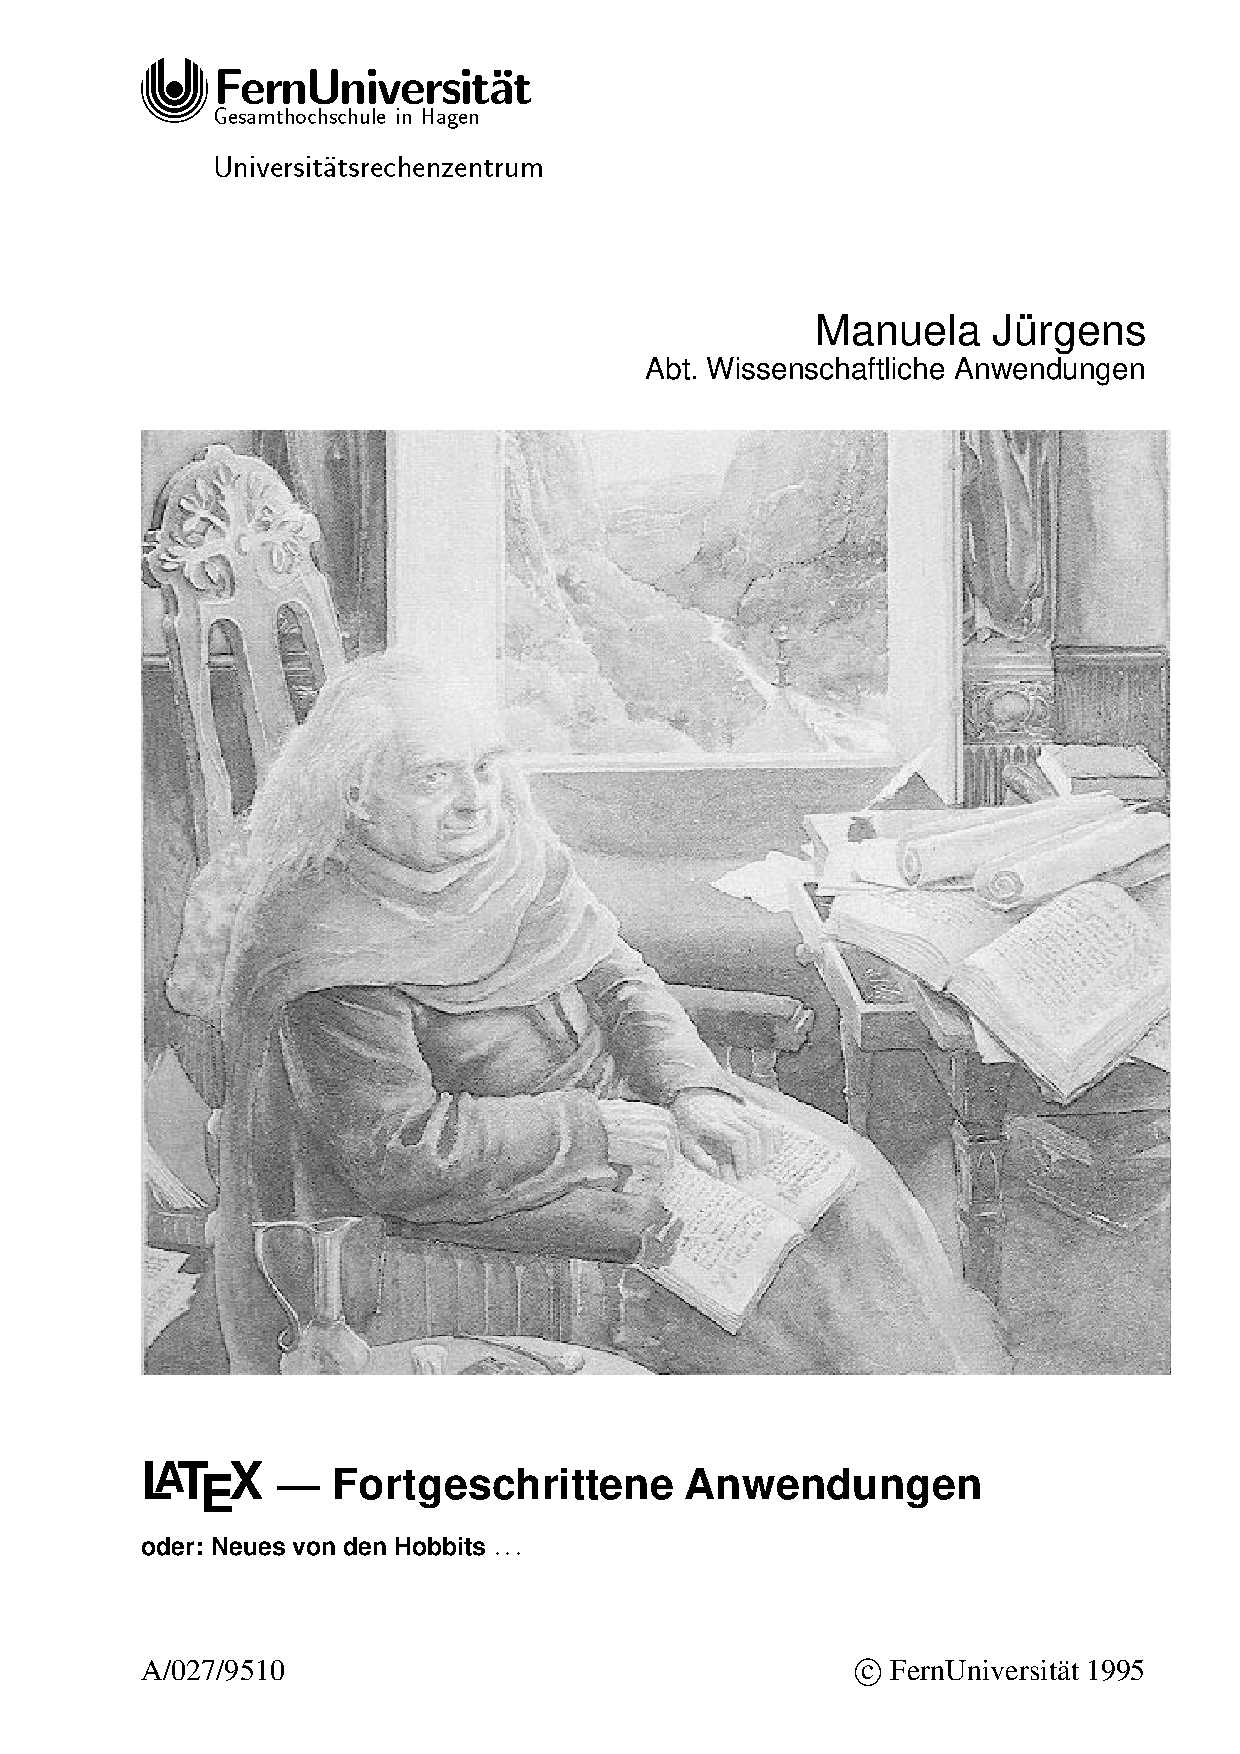
\includepdf[scale=1,page=-]{appendix/latex_2.pdf}
%
%
%
%%%%%%%%%%%%%%%%%%%%%%%%%%%%%%%%%%%%%%%%%%%%%%%%%%%%%%%%%%%%%%%%%%%%%%%%%%%%%%%
% Stichwortverzeichnis
%%%%%%%%%%%%%%%%%%%%%%%%%%%%%%%%%%%%%%%%%%%%%%%%%%%%%%%%%%%%%%%%%%%%%%%%%%%%%%%
\renewcommand{\indexname}{Stichwortverzeichnis} 
\printindex
%
%
%
\end{document}
